\documentclass[12pt]{article}


\usepackage{graphicx}
\usepackage{amsmath, amsfonts}

\graphicspath{ {paper_figures/PCA_analysis/} }
\usepackage{epstopdf}

\usepackage[margin=1in]{geometry}

\begin{document}


\begin{figure}
\begin{minipage}{5.1cm}
\centering
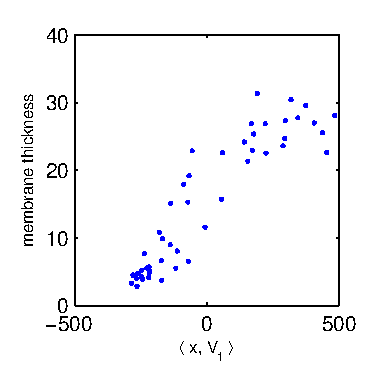
\includegraphics[width=5cm]{PCA_membrane_corr} \\
(a)
\end{minipage}
\begin{minipage}{5.1cm}
\centering
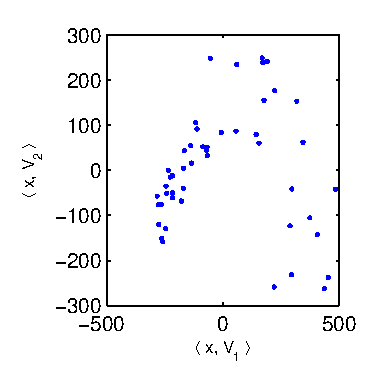
\includegraphics[width=5cm]{PCA_12}\\
(b)
\end{minipage}
\begin{minipage}{5.1cm}
\centering
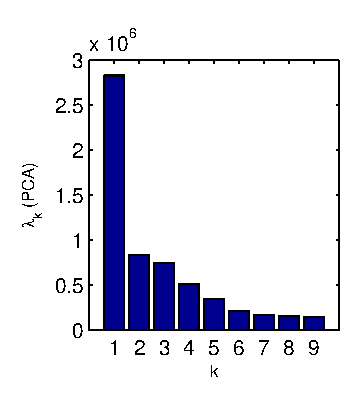
\includegraphics[width=5cm]{evals}\\
(c)
\end{minipage}\\
\begin{minipage}{12.5cm}
\centering\

\includegraphics[width=3cm]{eigenimage_1}
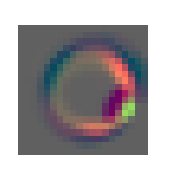
\includegraphics[width=3cm]{eigenimage_2}
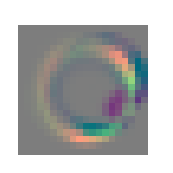
\includegraphics[width=3cm]{eigenimage_3}

\includegraphics[width=3cm]{eigenimage_4}\\
(d)
\end{minipage}\\
\begin{minipage}{6.2cm}
\centering
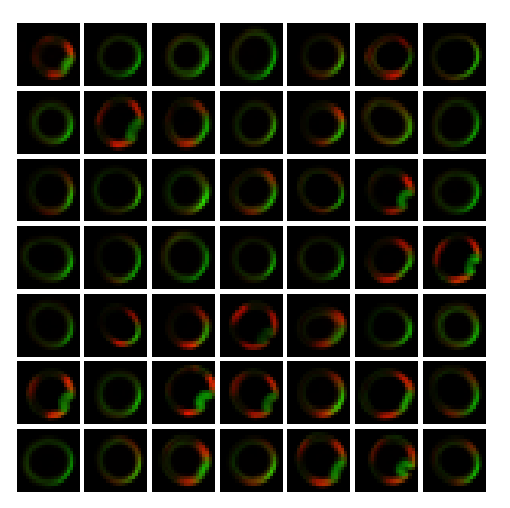
\includegraphics[width=6cm]{image_array}\\
(e)
\end{minipage}
\begin{minipage}{6.2cm}
\centering
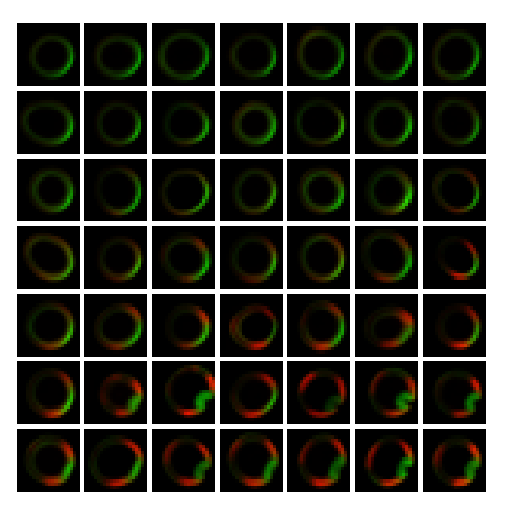
\includegraphics[width=6cm]{image_array_ordered}\\
(f)
\end{minipage}
\caption{(a) Membrane thickness versus first PCA projection coefficient. (b) PCA projection 1 versus 2. (c) PCA eigenvalue spectrum. (d) First 4 PCA eigenimages. (e) Images, registered (using angular synchronizaton), but unordered. (f) Images, ordered by first PCA projection coefficient. }
\end{figure}

\end{document}